Taking one of the formulations defined in previous experiments, a functional validation prototype was constructed to evaluate the audio-to-voltage transduction and signal attenuation in the gelatine medium.

\paragraph*{Prototype Fabrication}
A dedicated phantom cube was fabricated with an embedded audio interface (3.5mm Mono Jack) positioned centrally within the conductive volume as shown in Figure~\ref{fig:gelatine_prototype_3}. This allowed for the direct injection of analog audio signals into the medium.

\begin{figure}[H]
    \centering
    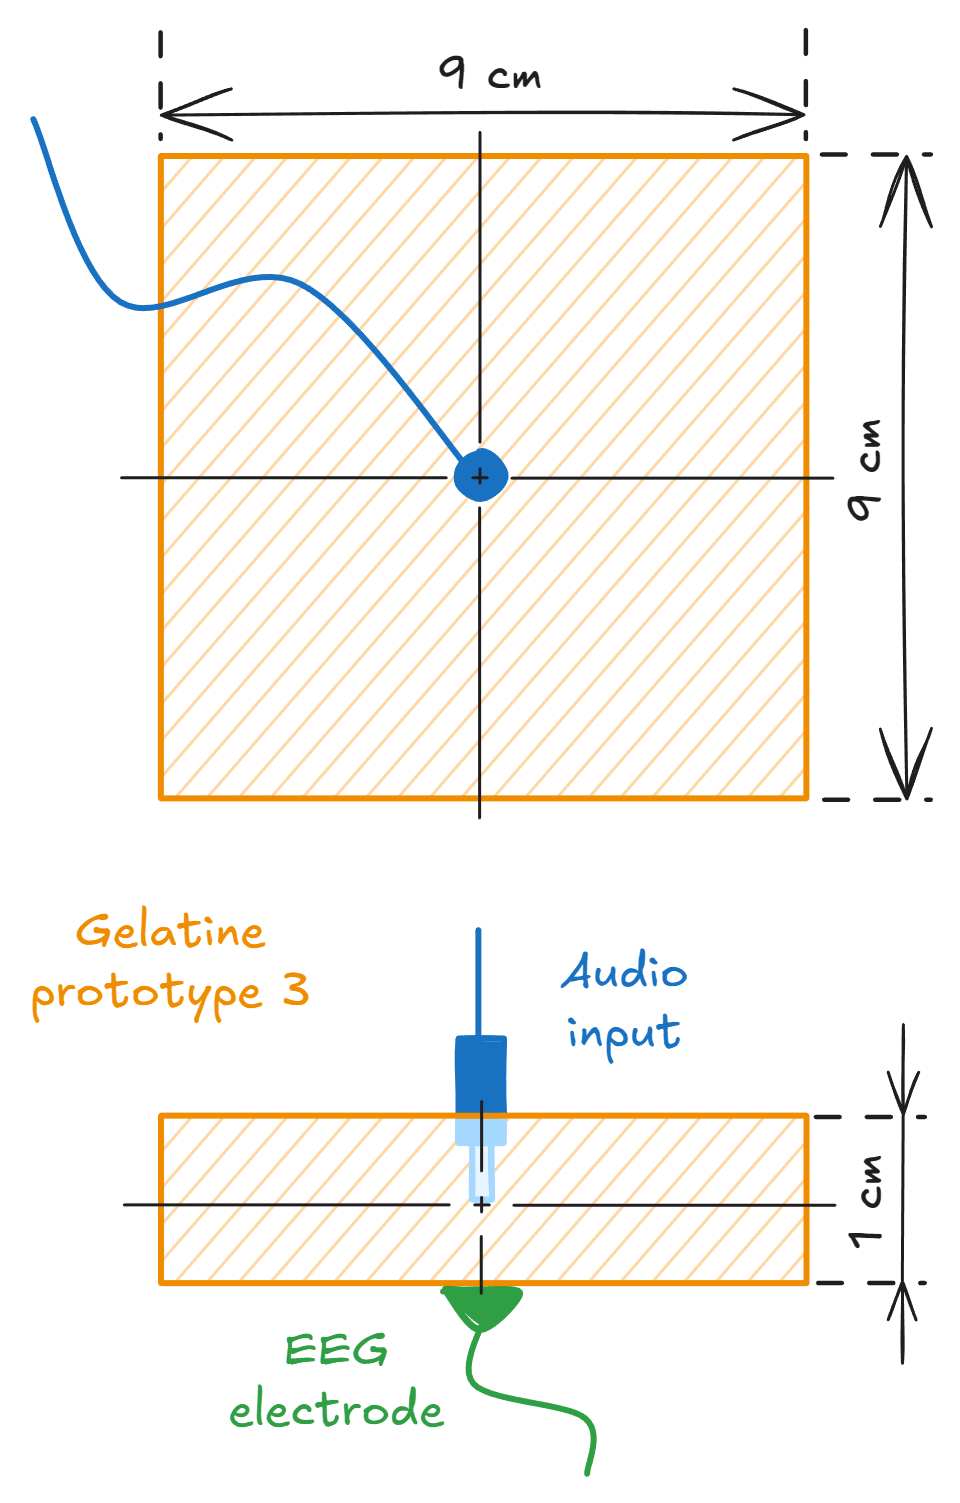
\includegraphics[width=0.6\textwidth]{../../02_Images/gelatine_prototype_3.png}
    \caption[Gelatine prototype for audio-to-voltage transduction]{Gelatine prototype for audio-to-voltage transduction.}
    \label{fig:gelatine_prototype_3}
\end{figure}

\begin{figure}[H]
    \centering
    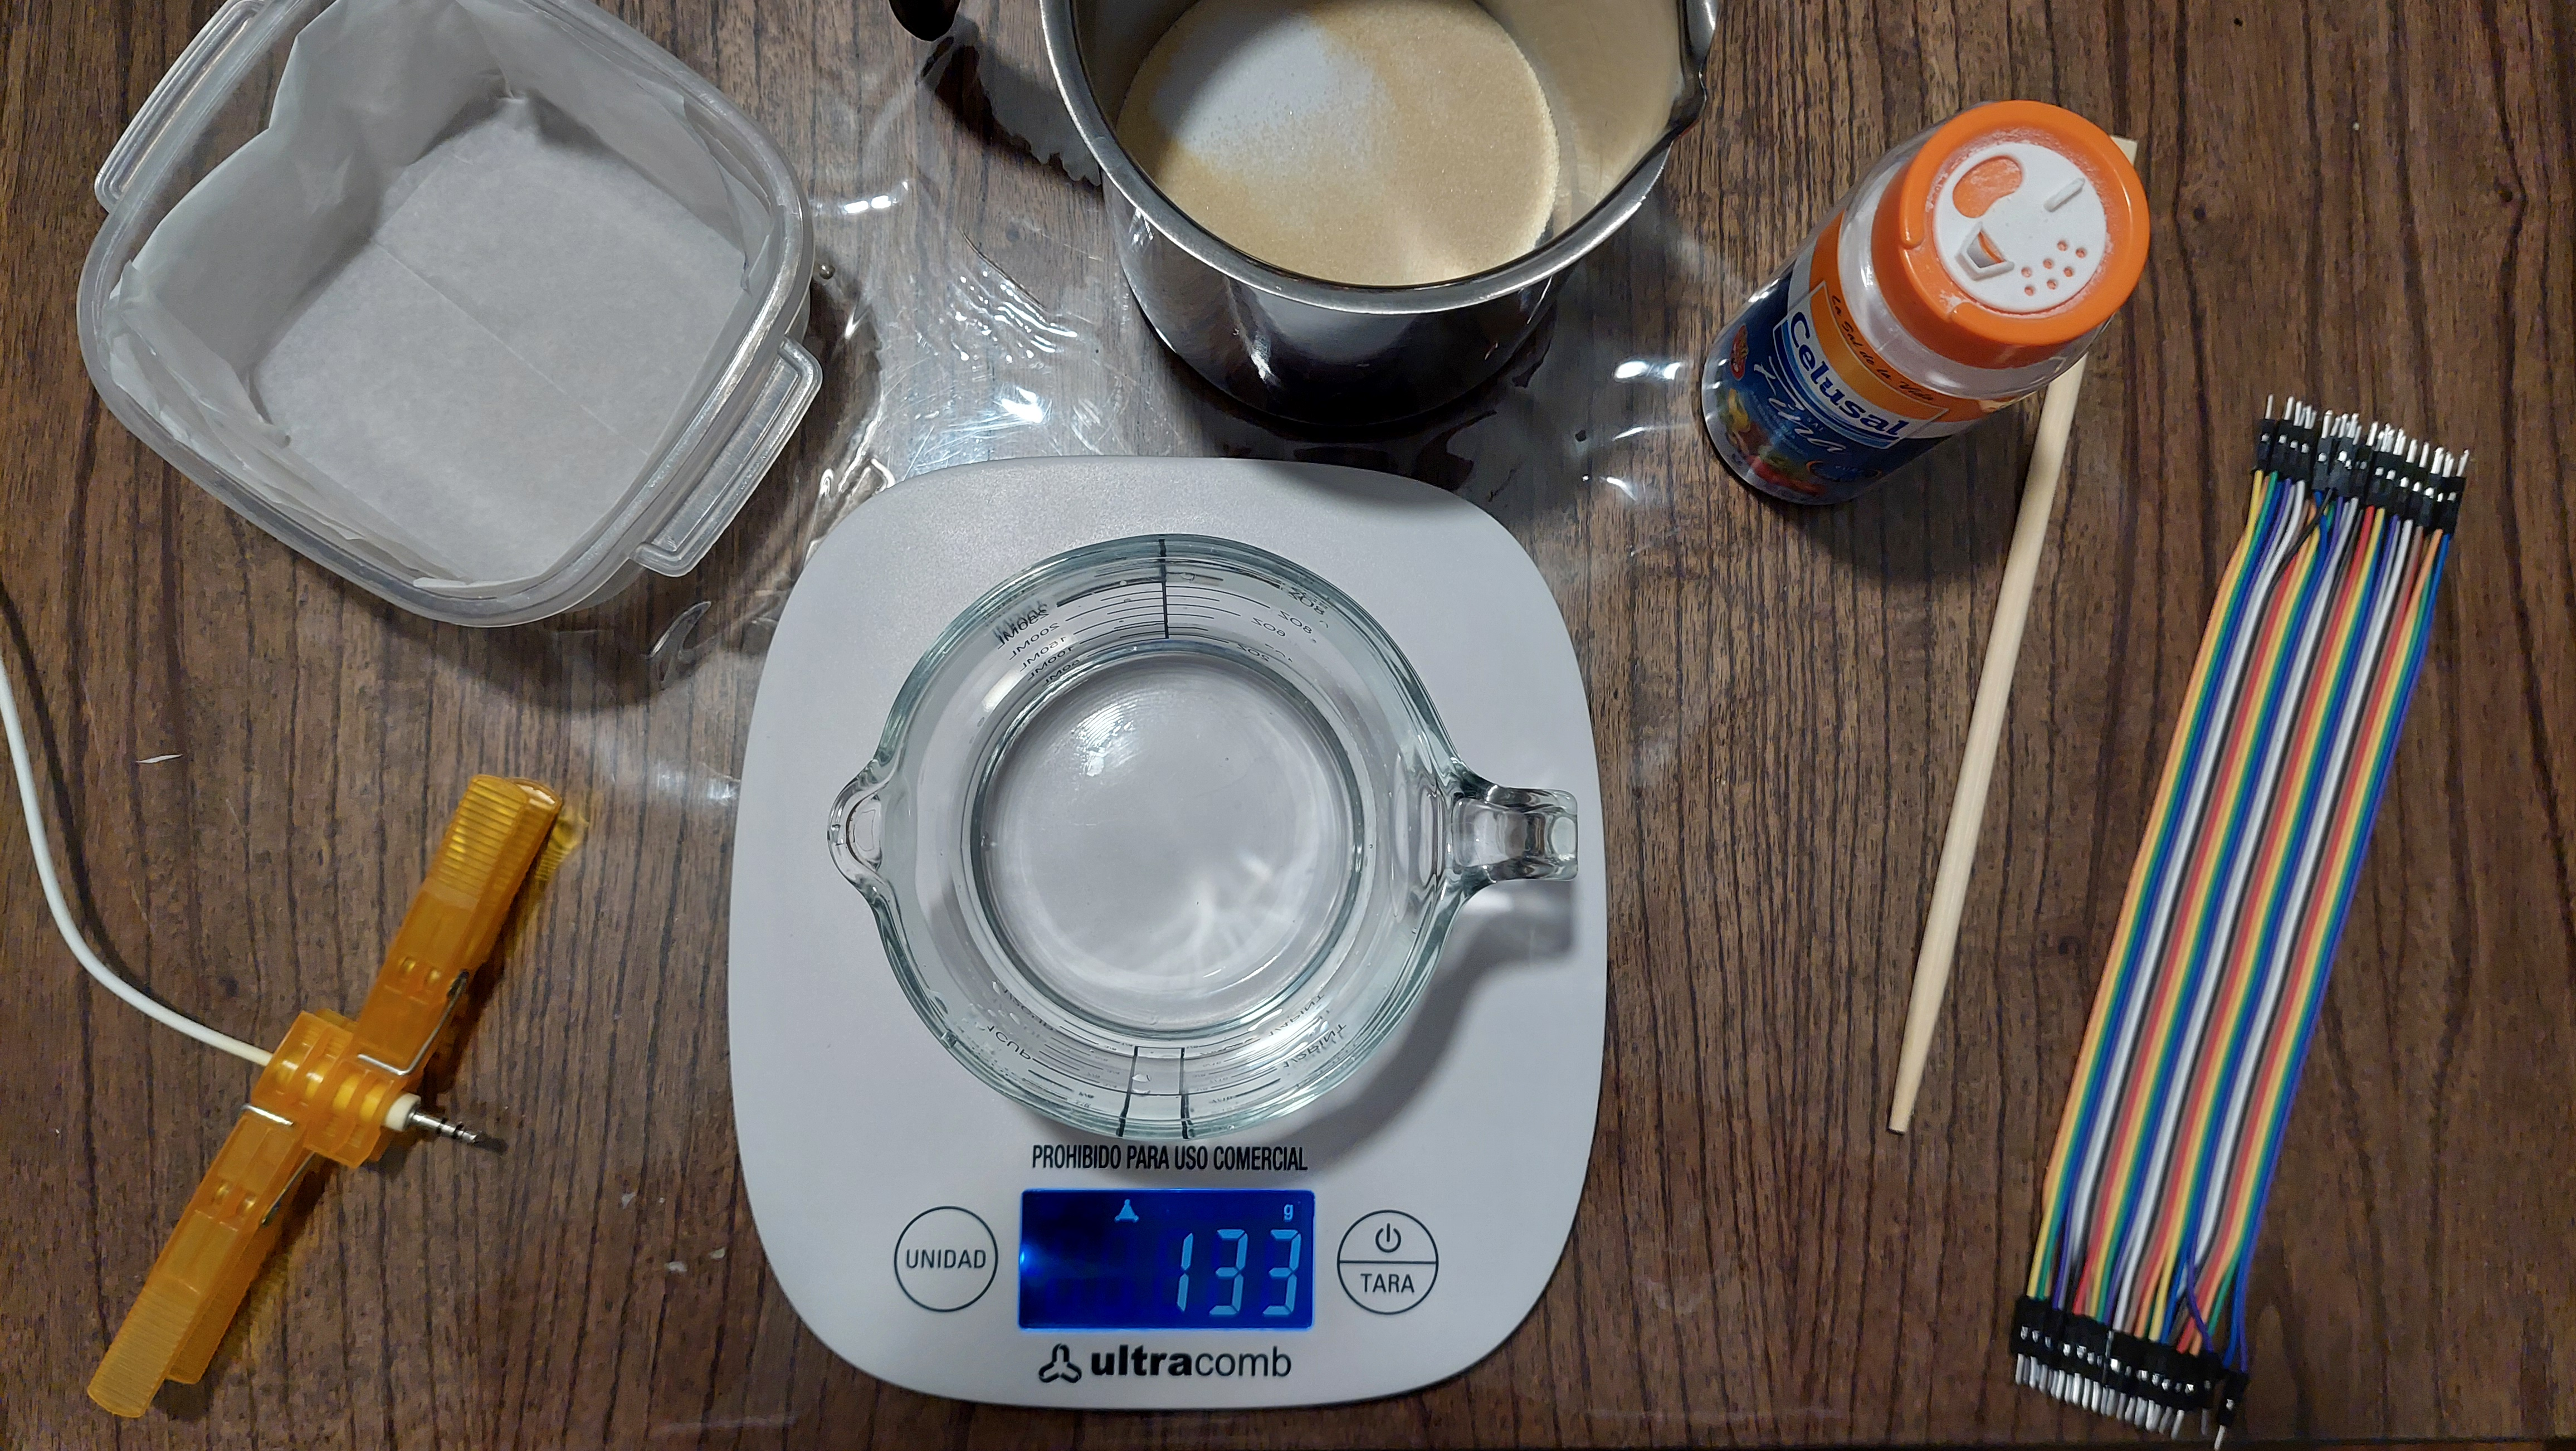
\includegraphics[width=0.6\textwidth]{../../02_Images/transduction_ingredients.jpg}
    \caption[Transduction Ingredients]{Ingredients for audio-to-voltage transduction experiment within the gelatine phantom.}
    \label{fig:transduction_ingredients}
\end{figure}

\subsubsection{Experiment 4: Signal Transduction and Attenuation}
The objective of this experiment is to validate the audio-to-voltage transduction approach as a viable method for generating bioelectric potentials within the phantom structure. By injecting known audio signals and measuring the resulting voltage at the surface, we can observe the attenuation introduced by the medium.

The experiment utilized two distinct signal sources for comparison:
\begin{enumerate}
    \item \textbf{Reference Source:} A verified third-party mobile application (Frequency Sound Generator) with a high user rating, used to establish a baseline for sine wave fidelity.
    \item \textbf{Our Software Platform:} The proprietary software developed for this thesis.
\end{enumerate}

The output signals were acquired using an \gls{eeg} electrode connected to a \textbf{OpenBCI Cyton} biosensing board. The signals were visualized and logged using the proprietary OpenBCI \gls{gui} to verify frequency accuracy and measure the peak-to-peak voltage attenuation introduced by the medium.

\begin{figure}[h]
    \centering
    \includegraphics[width=0.6\textwidth]{../../02_Images/transduction_setup.png}
    \caption[Transduction Setup]{Setup for audio-to-voltage transduction experiment within the gelatine phantom.}
    \label{fig:transduction_setup}
\end{figure}